\chapter{Hello Adventure World} 

\section{Introduction}

A program is basically a set of instructions what to do. There are different programming languages we can write such instructions in -- Python is one of them. Other languages are for example Java, C, C++, Swift -- by now (October 2018) probably close to 300 different programming languages exist! But, we will just focus on Python for the moment. 

Python is actually more than "just" a language. It is also a program that can interpret your program and then translate it into instructions for your computer to execute. Let us see that in action right away. 

Open a terminal, type in \textbf{\texttt{idle3 \&}} after the \$-prompt, and press return: 

\begin{itemize}
\item[\$] \textbf{\texttt{idle3 \&}}
\end{itemize}

Up pops a little window, like the one below.  
 
\begin{figure}[h]
\centerline{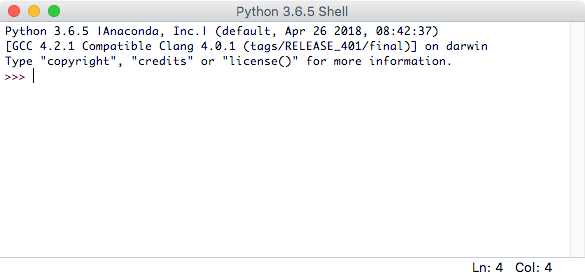
\includegraphics[scale=.70]{images/p1ch1-idle3.png}}
\caption{The Python IDLE3 interactive editor}
\end{figure}

This is the \texttt{idle3} window. It is an interactive editor for Python. Everything you type in is immediately interpreted and executed -- so you can see right away what it does! 
Let's see this at work. After the "$>>>$" prompt in the editor, type in the following: 

\begin{itemize}
\item[$>>>$] \textbf{\texttt{print("Hello adventure world!")}}
\end{itemize}



 